\section{Design of \name}
\label{sec:dda:design}

In this section, we present the \name approach that yields accurate throughput prediction (Section~\ref{sec:dda:eval}). 
We start with an intuitive description of \name before formally describing the algorithm.



\subsection{Insight of \name}

At a high level, \name finds for any session $\session$ a {\em prediction model} -- a pair of features and time range, which is used to aggregate history sessions that match the specific features with $\session$ and happened in the specific range. 
%Intuitively, we want the aggregated history sessions to have similar throughput with $\session$ so that they can produce a highly accurate prediction.

To motivate how \name maps a session to a prediction model, let us consider two strawmen of session-model mapping shown in Figure~\ref{fig:tbd-motivation}. 
The first strawman maps each session $\session$ to the ``Nearest Neighbor'' prediction model (dash arrows), which aggregates only history sessions matching all features with $\session$ and happening in very short time (e.g., 5 minute) before $\session$. Theoretically, ``Nearest Neighbor'' model should be highly accurate as it represents sessions that are the most similar to $\session$, but history sessions meeting this requirement are too sparse to provide reliable prediction. 
Alternatively, one can map any $\session$ to the ``Global'' prediction model (dot arrows), which aggregates all history sessions regardless of their features or happening time. While ``Global'' model is highly reliable as it has substantial samples in history, the accuracy is low because it does not capture the effect of feature combination introduced in the last section. 


\begin{figure}[t!]
\centering
%\vspace{-0.4cm}
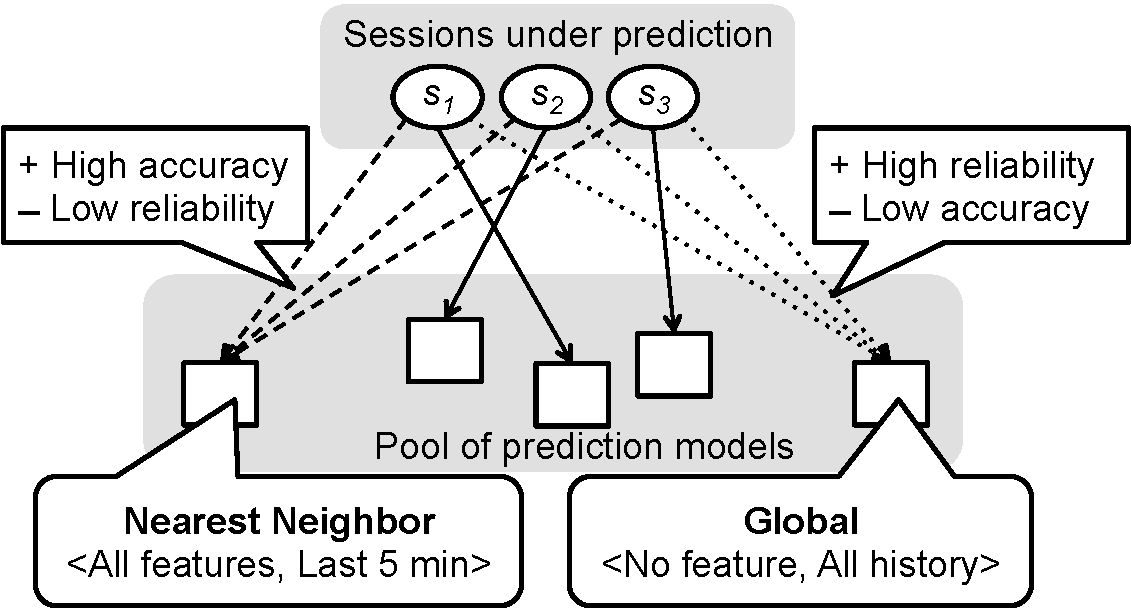
\includegraphics[width=0.7\textwidth]{figures/dda-tbd-motivation.pdf}
\caption{Mapping between sessions under prediction and prediction models.}
\label{fig:tbd-motivation}
\end{figure}

Ideally, we would like achieve both high accuracy and high reliability. To this end, \name (shown by solid arrows in Figure~\ref{fig:tbd-motivation}) differs from the above strawmen in two important aspects. First, \name finds for a given session a prediction model between the Nearest Neighbor and Global prediction models, so that it  strikes a balance between being closer to Nearest Neighbor for accuracy and being closer to Global for reliability. The resulting prediction model should be expressive (e.g., have more features) and yet have enough samples to offer a reliable prediction.
Second, instead of mapping all sessions to the same prediction model, \name maps different sessions to different prediction models, which allows \name to address inherent heterogeneity that the same feature has different impact on different sessions.


\subsection{Algorithm}

\mypara{Overall workflow} \name uses two steps to predict the throughput of a new session $\session$.
\begin{packedenumerate}
\item First, \name learns a prediction model $\Model^{\optimal}_\session$ based on history data. A prediction model is a pair of feature combination and time range. 
\item Second, \name estimates $\session$'s throughput by the median throughput of sessions in $\Agg{\Model^{\optimal}_\session}{\session}$ that match $\session$ on the feaures of $\Model^{\optimal}_\session$ and are in the time range of $\Model^{\optimal}_\session$. I.e., \name's prediction is $\Pred{\session}=\QualitySummary(\Agg{\Model^{\optimal}_\session}{\session})$.
\end{packedenumerate}


\mypara{Learning of prediction model} First, \name learns a prediction model $\Model^{\optimal}_\session$ based on history data from a pool of all possible prediction models, i.e., pairs of all feature combinations (i.e., $2^n$ subsets of $n$ features in Table~\ref{tab:fcc-stats}) and possible time windows. Specifically, the possible time windows include time windows of certain history length (i.e., last 10 minutes to last 10 hours) and those of same time of day/week (i.e., same hour of day in the last 1-7 days or same hour of week in the last 1-3 weeks). 

The objective of $\Model^{\optimal}_\session$ is to minimize the prediction error, $\Error{\Pred{\session}}{\Throughput{\session}}=\frac{|\Pred{\session}-\Throughput{\session}|}{\Throughput{\session}}$, where  $\Throughput{\session}$ is the actual throughput of $\session$. That is,


%We start with \name's workflow to predict throughput of session $\session$:
%\begin{packedenumerate}
%\item First, \name picks a prediction model $\Model^{\optimal}_\session$ from a pool of all prediction models, i.e., pairs of all feature combinations (i.e., $2^n$ subsets of $n$ features in Table~\ref{tab:fcc-stats}) and time windows. Specifically, the possible time windows include time windows of certain history length (i.e., last 10 minutes to last 10 hours) and those of same time of day/week (i.e., same hour of day in the last 1-7 days or same hour of week in the last 1-3 weeks). 
%\item Second, once prediction model $\Model^{\optimal}_\session$ is picked for $\session$, \name aggregates history sessions based on $\Model^{\optimal}_\session$. For instance, given $\Model^{\optimal}_\session=\Pair{ISP}{1hr}$, \name will aggregate all history sessions who are in the same ISP with $\session$ and happened in the last 1 hour. Formally, this set of history sessions denoted by $\Agg{\Model^{\optimal}_\session}{\session}$.
%\item Finally, \name predicts the throughput of $\session$ by $\Pred{\session}=\QualitySummary(\Agg{\Model^{\optimal}_\session}{\session})$, where $\QualitySummary(S)$ reports the median of the throughput of sessions in $S$.
%\end{packedenumerate}
%
%The goal of $\Pred{\session}$ is to minimize the prediction error $\Error{\Pred{\session}}{\Throughput{\session}}=\frac{|\Pred{\session}-\Throughput{\session}|}{\Throughput{\session}}$, where  $\Throughput{\session}$ is the actual throughput of $\session$

%{\footnotesize
%\vspace{-0.4cm}
\begin{align}
&\Model^{\optimal}_\session=\argmin_{\Model}
\Error{\QualitySummary(\Agg{\Model}{\session})}{\Throughput{\session}} \label{eq:goal}
\end{align}
%\vspace{-0.4cm}
%}

\noindent Rather than solving Eq~\ref{eq:goal} analytically, \name takes a {\em data-driven} approach and finds the best prediction model over a set of history sessions $\Estimation{\session}$ (defined shortly). Formally, the process can be written as following:

%{\footnotesize
%\vspace{-0.4cm}
\begin{align}
&\Model^{\optimal}_\session=\argmin_{\Model}\frac{1}{|\Estimation{\session}|}\sum_{\session'\in\Estimation{\session}}
\Error{\QualitySummary(\Agg{\Model}{\session'})}{\Throughput{\session'}} \label{eq:empirical}
\end{align}
%\vspace{-0.4cm}
%}

\noindent$\Estimation{\session}$ should include sessions that are likely to share the best prediction model with $\session$. In \name, $\Estimation{\session}$ consists of sessions that match features $\mathit{Target}$, $\mathit{ISP}$, $\mathit{Technology}$ and $\mathit{Downlink}$ with $\session$ and happened within 4 hours before $\session$. 


\mypara{Estimating throughput} Second, \name estimates $\session$'s throughput by the learned prediction model $\Model^{\optimal}_\session$.
%\name also adopts two fine-grain optimizations to further improve corner cases. First, 
To make the prediction $\Pred{\session}$ reliable, \name ensures that $\Pred{\session}$ is based on a substential amount of sessions in $\Agg{\Model^{\optimal}_\session}{\session}$. Therefore, if $\Model^{\optimal}_\session$ yields $\Agg{\Model^{\optimal}_\session}{\session}$ with less than 20 sessions, \name will remove that model from the pool and learn the prediction model as in the first step again.
%Second, 
We have also found that for some pairs of client and server, \name's prediction error is one-sided. For instance, the throughput of a particular client-server pair is 1Mbps, while the best prediction model always predicts 2Mbps (i.e., a one-sided 100\% error). We compensate this error by changing $\QualitySummary(S)$ to $\QualitySummary(S,k)$ which reports the median of throughput in $S$ times a factor $k$. To train a proper value of $k$, \name first uses Eq~\ref{eq:empirical} to learn $\Model^{\optimal}_\session$ by assuming $k=1$, and then, \name trains the best factor $k^{\optimal}_\session$ for $\session$ as follows: 

%{\footnotesize
%\vspace{-0.4cm}
\begin{align}
&k^{\optimal}_\session=\argmin_{k}\frac{1}{|\Estimation{\session}|}\sum_{\session'\in\Estimation{\session}}
\Error{\QualitySummary(\Agg{\Model^{\optimal}_\session}{\session'},k)}{\Throughput{\session'}} \nonumber
\end{align}
%\vspace{-0.4cm}
%}

\noindent where $k$ is chosen from 0 to 5. Finally, the prediction made by \name will be $\QualitySummary(\Agg{\Model^{\optimal}_\session}{\session},k^{\optimal}_\session)$.



